\section{WERYFIKACJA PRACY PROGRAMU}

\subsection{Testy jednostkowe}

Działanie wszystkich funkcji wchodzących w skład logiki biznesowej programu
zostało zweryfikowane testami jednostkowymi. Wynik wykonania testów
jednostkowych można zobaczyć na listingu \ref{cargoTestListing}.

\lstinputlisting[
    float=h!,
    frame=tb,
    label={cargoTestListing},
    caption={Wykonanie testów jednostkowych}
]{./code/cargoTest.txt}

\subsection{Testy integracyjne}

Działanie niektórych funkcji programu jest zależne od bazy danych. Weryfikacja
działania tych funkcji za pomoca testów jednostkowych wymagałaby napisania dużej
ilości serwisów mock. Z tego powodu, przetestowanie tych funkcji programu, jak i
tych, które posiadają testy jednostkowe przeprowadzono za pomocą testów
integracyjnych.

Testy integracyjne zostały napisane w programie Postman. Jest to program służący
do testowania API. Testy napisane w tym programie można wyeksportować do pliku
json, który można wykonać z poziomu powłoki tekstowej za pomocą programu
newman. Pozwala to na automatyczne wykonywanie testów.

Wykonanie testów integracyjnych widać na rysunku \ref{postmanTestExec}.

\begin{figure}[h]
    \centering
    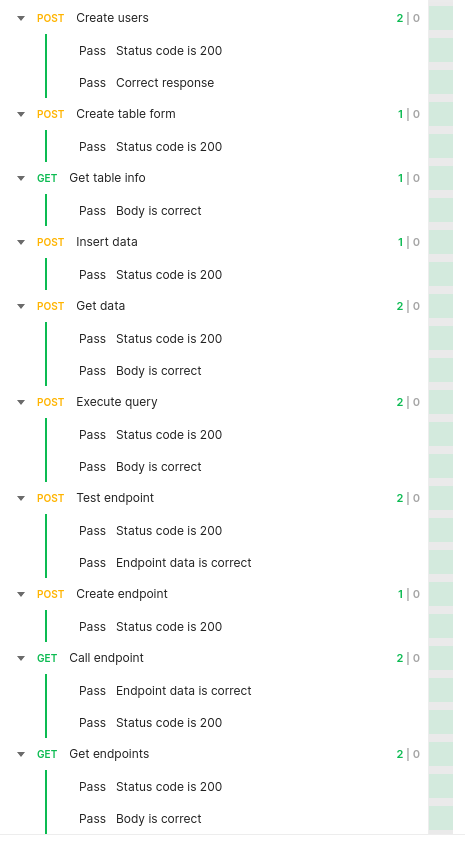
\includegraphics[width=0.6\textwidth]{./img/postman_test_exec.png}
    \caption{Wykonanie testów integracyjnych w programie Postman}
    \label{postmanTestExec}
\end{figure}
